\section{第十一周数值分析实验}
\subsection{牛顿一科特斯积分}
\begin{ex}
	编写牛顿一科特斯积分公式程序, 思路如下:
	
	(1) 对区间 $[a, b]$ 作 $n$ 等份, 确定数值点 $x_k$, 求解被积函数的函数值 $y_k=f\left(x_k\right)$;
	
	(2) 计算第 $k$ 个科特斯系数 $C_k^{(n)}=\frac{(-1)^{n-k}}{n k !(n-k) !} \int_0^n \prod_{\substack{j=0 \\ j \neq k}}^n(t-j) \mathrm{d} t$
	
	(3) 构造牛顿一科特斯积分公式 $\int_a^b f(x) d x=(b-a) \sum_{k=0}^n C_k^{(n)} f\left(x_k\right)$.
	
	(4) 利用 $M A T L A B$ 编写算法实现, 参考函数格式为:
	$$
	I_{\text {out }}=\text { NewtonCotesIntegration }(f, a, b, n)
	$$
\end{ex}
\lstinputlisting[language=matlab]{w11/NewtonCotesIntegration.m}
\subsection*{例子}
\begin{ex}
	利用程序计算下列两个积分
	$$
	I_1=\int_1^9 \sqrt{x} d x \quad \text { 及 } \quad I_2=\int_0^2 \sqrt{4-x^2} \mathrm{~d} x
	$$
	并比较结果
	1. 梯形公式;2. 辛普森公式;3. 科特斯公式.
\end{ex}
\lstinputlisting[language=matlab]{w11/q2.m}
\begin{ex}
	选择尽可能精确的方法计算下列积分
	$$
	S=a \int_0^{\pi / 2} \sqrt{1-\left(\frac{c}{a}\right)^2 \sin ^2 \theta} d \theta
	$$
	其中
	$$
	\begin{aligned}
		& a=(2 R+H+h) / 2, c=(H-h) / 2, \\
		& R=6371, \quad H=2384, \quad h=439
	\end{aligned}
	$$
\end{ex}
\begin{figure}[H]
	\centering
	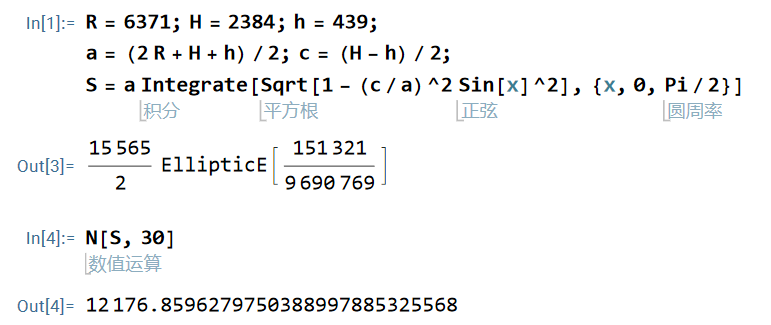
\includegraphics[width = 0.8\linewidth]{w11/fig.png}
	\caption{Mathematica结果}
\end{figure}
\lstinputlisting[language=matlab]{w11/q3.m}
\begin{figure}[H]
	\centering
	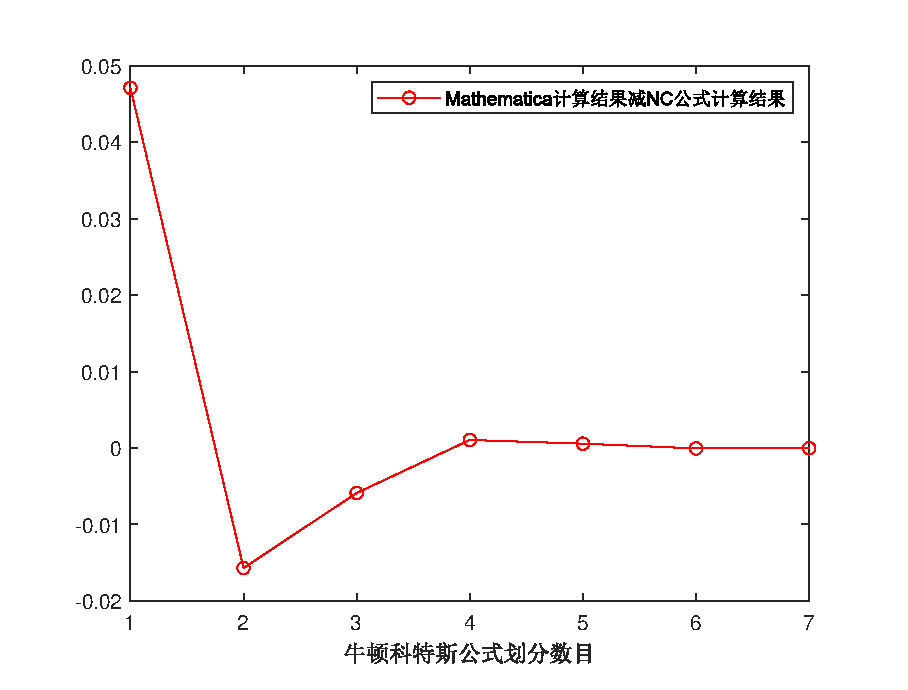
\includegraphics[width = 0.61\linewidth]{w11/fig.eps}
	\caption{结果比较}
\end{figure}

